\documentclass[a4paper, czech]{article}

\usepackage[czech]{babel}
\usepackage{indentfirst}
\usepackage{graphicx}
\usepackage{float}
\usepackage[margin=1.5cm]{geometry}
\usepackage{booktabs}
\usepackage{amsmath}
\usepackage{xcolor}
\usepackage{multirow}
\usepackage{tabularray}
\usepackage{bold-extra}
\usepackage{circuitikz}

\begin{document}
\begin{table}[H]
    \centering
    \begin{tblr}{
        cell{1}{1} = {c = 2, r = 4}{c}, % Logo
        cell{1}{4} = {c = 3}{c}, % Předmět
        cell{2}{4} = {c = 3}{c}, % Jméno
        cell{3}{4} = {}{c}, % Ročník
        cell{3}{6} = {}{c}, % Studijní skupina
        cell{4}{4} = {}{c}, % Spolupracoval
        cell{4}{6} = {}{c}, % Mereno dne
        cell{5}{1} = {c = 2}{55mm}, % Kontroloval
        cell{5}{3} = {c = 2}{55mm}, % Hodnoceni
        cell{5}{5} = {c = 2}{55mm}, % Dne
        cell{6}{2} = {c = 5}{}, % Nazev ulohy
        cell{7}{1} = {}{c}, % Číslo úlohy
        cell{7}{2} = {c = 5}{c}, % Název úlohy
        vline{1,2,7} = {1.2pt},
        vline{3,5},
        hline{1,5,6,8} = {1.2pt},
        hline{2,3,4}
        }
        
\includegraphics{logo_fekt.png} & & \textsuperscript{Předmět} & \large \textbf{Měření v audiotechnice} \\
             & & \textsuperscript{Jméno} & \large \textbf{Karolína Šebestová} \\
             & & \textsuperscript{Ročník} & \large \textbf{3.} & \textsuperscript{Studijní skupina} & \large \textbf{St 14:00} \\
             & & \textsuperscript{Spolupracoval} & \large \textbf{Filip Kokavec} & \textsuperscript{Měřeno dne} & \large \textbf{30.10.2024} \\
        \textsuperscript{Kontroloval} & & \textsuperscript{Hodnocení} & & \textsuperscript{Dne} \\
        \textsuperscript{Číslo úlohy} & \textsuperscript{Název úlohy} \\
        \Large \textbf{5A AUDIO} & \Large \textsc{\textbf{Automatizované měření vlastností audio zesilovače}} \\
    \end{tblr}
\end{table}

\section{Zadání}

\begin{itemize}
    \item Pomocí programu v prostředí Keysight VEE změřte kmitočtovou charakteristiku modulu a fáze přenosu zesilovače.
    \item Pomocí osciloskopu změřte spektrum výstupního signálu ze zesilovače buzeného harmonickým signálem a vypočí- tejte hodnotu činitele harmonického zkreslení.
    \item Změřte úroveň přeslechů v zesilovači z kanálu 1 do kanálu 2.
    \item Změřte a vypočítejte úroveň odstupu signálu od šumu a rychlost přeběhu.
\end{itemize}

\section{Teoretický úvod}

\begin{figure}[H]
    \centering
    \begin{circuitikz}
        \draw[thick] (0,0) to (5,0) to (5,-3) node[ocirc, scale=2](CH11){}
        to (5,-3.5) node[ocirc, scale=2](CH12){}
        to (5,-4.5) node[ocirc, scale=2](CH21){}
        to (5,-5) node[ocirc, scale=2](CH22){}
        to (5,-6) to (0,-6) to (0,-4.5) node[ocirc, scale=2](GEN2){}
        to (0,-5) node[ocirc, scale=2](GEN1){}
        to (0,0);

        \draw (2.5,-7.5) node[fourport](AMP){};

        \draw[thick] (CH21) to ++(0.5,0) coordinate(Aport3) to (Aport3 |- AMP.port3) to (AMP.port3) node[ocirc, scale=2]{};
        \draw[thick] (CH22) to ++(1,0) coordinate(Aport2) to (Aport2 |- AMP.port2) to (AMP.port2) node[ocirc, scale=2]{};

        \draw[thick] (CH11) to ++(0.5,0) to ++(0,3.5) to ++(-6,0) coordinate(Aport4) to (Aport4 |- AMP.port4) to (AMP.port4) node[ocirc, scale=2]{};
        \draw[thick] (CH12) to ++(1,0) to ++(0,4.5) to ++(-7,0) coordinate(Aport1) to (Aport1 |- AMP.port1) to (AMP.port1) node[ocirc, scale=2]{};

        \draw[thick] (GEN2) to[] (GEN2 -| Aport4) node[circ]{};
        \draw[thick] (GEN1) to[] (GEN1 -| Aport1) node[circ]{};

        \draw (AMP) node[ampshape]{} ++(0,6) node[]{\Large \textbf{OSCILOSKOP}};
        \draw (AMP) ++(2,0) node[]{CH1 výst} ++(-4,0) node[]{CH1 vst};
        \draw (GEN1) ++(1,0.25) node[]{GEN výst};
        \draw (CH11) ++(-0.5,-0.25) node[]{CH1};
        \draw (CH21) ++(-0.5,-0.25) node[]{CH2};

        \draw[thick, dashed] (5,-0.5) coordinate(USB) to ++(3,0) to ++(0,-1) coordinate(RECT_POS);
        \draw[thick] (RECT_POS) ++(-1,0) rectangle ++(2,-1) node[pos=0.5]{\Large \textbf{PC}};
        \draw (USB) ++(-0.5,0) node[]{USB};
    \end{circuitikz}
    \caption{Schéma zapojení pro měření kmitočtových charakteristik}
\end{figure}

\begin{figure}[H]
    \centering
    \begin{circuitikz}
        \draw[thick] (0,0) to (5,0) to (5,-3) node[ocirc, scale=2](CH11){}
        to (5,-3.5) node[ocirc, scale=2](CH12){}
        to (5,-4.5) node[ocirc, scale=2](CH21){}
        to (5,-5) node[ocirc, scale=2](CH22){}
        to (5,-6) to (0,-6) to (0,-4.5) node[ocirc, scale=2](GEN2){}
        to (0,-5) node[ocirc, scale=2](GEN1){}
        to (0,0);

        \draw (2.5,-7.5) node[fourport](AMP){};

        \draw[thick] (CH21) to ++(0.5,0) coordinate(Aport3) to (Aport3 |- AMP.port3) to (AMP.port3) node[ocirc, scale=2]{};
        \draw[thick] (CH22) to ++(1,0) coordinate(Aport2) to (Aport2 |- AMP.port2) to (AMP.port2) node[ocirc, scale=2]{};

        \draw[thick] (GEN2) to ++(-0.5,0) coordinate(Bport4) to (Bport4 |- AMP.port4) to (AMP.port4) node[ocirc, scale=2]{};
        \draw[thick] (GEN1) to ++(-1,0) coordinate(Bport1) to (Bport1 |- AMP.port1) to (AMP.port1) node[ocirc, scale=2]{};

        \draw (AMP) node[ampshape]{} ++(0,6) node[]{\Large \textbf{OSCILOSKOP}};
        \draw (AMP) ++(2,0) node[]{CH1 výst} ++(-4,0) node[]{CH1 vst};
        \draw (GEN1) ++(1,0.25) node[]{GEN výst};
        \draw (CH11) ++(-0.5,-0.25) node[]{CH1};
        \draw (CH21) ++(-0.5,-0.25) node[]{CH2};
    \end{circuitikz}
    \caption{Schéma zapojení pro měření
    harmonického zkreslení}
\end{figure}

\begin{figure}[H]
    \centering
    \begin{circuitikz}
        \draw[thick] (0,0) rectangle (3.5,-3) node[pos=0.5]{\Large \textbf{OSC}} ++(0,0.5) coordinate(GEN_VÝST);
        \draw[thick] (5,0) rectangle ++(5,-3) node[ampshape, pos=0.5, thin]{} ++(0,0.5) coordinate(CH2) ++(0,2) coordinate(CH1);

        \draw[thick] (GEN_VÝST) ++(0,0.25) node[ocirc, scale=2]{} to ++(0.5,0) to ++(0,2) to ++(1,0) node[ocirc, scale=2]{};
        \draw[thick] (GEN_VÝST) ++(0,-0.25) node[ocirc, scale=2]{} to ++(1,0) to ++(0,2) to ++(0.5,0) node[ocirc, scale=2]{};

        \draw[thick] (CH1) ++(0,0.25) node[ocirc, scale=2]{} to ++(1,0);
        \draw[thick] (CH1) ++(0,-0.25) node[ocirc, scale=2]{} to ++(1,0);

        \draw[thick] (CH2) ++(0,0.25) node[ocirc, scale=2]{} to ++(1,0);
        \draw[thick] (CH2) ++(0,-0.25) node[ocirc, scale=2]{} to ++(1,0);

        \draw (GEN_VÝST) ++(-1,0) node[]{GEN výst};
        \draw (CH1) ++(-1,0) node[align=right]{CH1 výst} ++(-3.15,0) node[align=left]{CH1 vst};
        \draw (CH2) ++(-1,0) node[align=right]{CH2 výst};

        \draw (11,-0.5) node[rmetershape, t=V, fill=white](V1){} ++(0,-2) node[rmetershape, t=V, fill=white](V2){};
    \end{circuitikz}
    \caption{Schéma zapojení pro měření mezikanálových přeslechů}
\end{figure}

\begin{figure}[H]
    \centering
    \begin{circuitikz}
        \draw[thick] (0,0) rectangle (3.5,-3) node[pos=0.5]{\Large \textbf{OSC}} ++(0,0.5) coordinate(GEN_VÝST);
        \draw (7,-1.5) node[fourport](AMP){} node[ampshape]{};
        \draw (10.5,-1.5) node[rmetershape, t=V](VOLTMETR){};

        \draw[thick] (GEN_VÝST) ++(0,0.25) node[ocirc, scale=2]{} to ++(0.5,0) coordinate(Cport4) to (Cport4 |- AMP.port4) to (AMP.port4) node[ocirc, scale=2]{};
        \draw[thick] (GEN_VÝST) ++(0,-0.25) node[ocirc, scale=2]{} to ++(1,0) coordinate(Cport1) to (Cport1 |- AMP.port1) to (AMP.port1) node[ocirc, scale=2]{};

        \draw[thick] (AMP.port3) node[ocirc, scale=2]{} to ++(0.5,0) to ++(0,0.5) coordinate(A) to (A -| VOLTMETR.north) to (VOLTMETR.north);
        \draw[thick] (AMP.port2) node[ocirc, scale=2]{} to ++(0.5,0) to ++(0,-0.5) coordinate(A) to (A -| VOLTMETR.south) to (VOLTMETR.south);

        \draw (GEN_VÝST) ++(-1,0) node[]{GEN výst};
        \draw (AMP.port4) ++(-0.8,-0.45) node[]{CH1 vst};
        \draw (AMP.port3) ++(0.8,-0.5) node[]{CH1 výst};
    \end{circuitikz}
    \caption{Schéma zapojení pro měření dynamického rozsahu}
\end{figure}

\pagebreak

\section{Výsledky měření}

\subsection{Tabulky}

\begin{table}[H]
    \catcode`\-=12
    \centering
    \caption{Automatizované měření kmitočtové charakteristiky zesilovače}
    \begin{tabular}{rcccc}
        \toprule
        \multicolumn{1}{c}{Kmitočet}   & \begin{tabular}[c]{@{}c@{}}Napětí na výstupu\\      generátoru\end{tabular} & \begin{tabular}[c]{@{}c@{}}Napětí na výstupu\\      zesilovače\end{tabular} & \begin{tabular}[c]{@{}c@{}}Modul\\      přenosu\end{tabular} & \begin{tabular}[c]{@{}c@{}}Fáze\\      přenosu\end{tabular} \\
        \cmidrule(rl){1-1}
        \cmidrule(rl){2-2}
        \cmidrule(rl){3-3}
        \cmidrule(rl){4-4}
        \cmidrule(rl){5-5}
        \multicolumn{1}{c}{$f$ {[}Hz{]}} & $U_g$ {[}V{]}                                                                  & $U_z$  {[}V{]}                    & Z {[}$\Omega${]}                                                    & $\phi$ {[}°{]}                                                   \\
        \midrule
        5          & 0,247                                                                       & 0,50                           & 6,125                                                        & -84,0                                                       \\
        7          & 0,247                                                                       & 0,56                           & 7,172                                                        & -60,4                                                       \\
        10         & 0,246                                                                       & 0,61                           & 7,845                                                        & -44,1                                                       \\
        15         & 0,246                                                                       & 0,64                           & 8,250                                                        & -29,4                                                       \\
        20         & 0,246                                                                       & 0,65                           & 8,440                                                        & -22,4                                                       \\
        30         & 0,246                                                                       & 0,66                           & 8,506                                                        & -14,6                                                       \\
        40         & 0,246                                                                       & 0,66                           & 8,572                                                        & -12,7                                                       \\
        60         & 0,246                                                                       & 0,66                           & 8,585                                                        & -6,5                                                        \\
        100        & 0,246                                                                       & 0,66                           & 8,572                                                        & -3,9                                                        \\
        200        & 0,246                                                                       & 0,66                           & 8,572                                                        & -2,8                                                        \\
        400        & 0,246                                                                       & 0,67                           & 8,703                                                        & -2,0                                                        \\
        600        & 0,246                                                                       & 0,67                           & 8,638                                                        & -1,8                                                        \\
        1 000       & 0,246                                                                       & 0,67                           & 8,703                                                        & -1,7                                                        \\
        2 000       & 0,246                                                                       & 0,67                           & 8,703                                                        & -1,0                                                        \\
        3 000       & 0,246                                                                       & 0,67                           & 8,638                                                        & -0,9                                                        \\
        4 000       & 0,246                                                                       & 0,67                           & 8,703                                                        & -1,2                                                        \\
        6 000       & 0,246                                                                       & 0,67                           & 8,638                                                        & -0,2                                                        \\
        10 000      & 0,246                                                                       & 0,67                           & 8,703                                                        & 0,9                                                         \\
        15 000      & 0,246                                                                       & 0,67                           & 8,664                                                        & 0,7                                                         \\
        20 000      & 0,246                                                                       & 0,67                           & 8,703                                                        & 2,1                                                         \\
        30 000      & 0,246                                                                       & 0,67                           & 8,729                                                        & 5,4                                                         \\
        40 000      & 0,246                                                                       & 0,64                           & 8,305                                                        & 18,2                                                        \\
        60 000      & 0,246                                                                       & 0,57                           & 7,344                                                        & 46,3                                                        \\
        100 000     & 0,245                                                                       & 0,40                           & 4,214                                                        & 80,9                                                        \\
        150 000     & 0,245                                                                       & 0,27                           & 0,747                                                        & 95,2                                                        \\
        200 000     & 0,244                                                                       & 0,20                           & -1,727                                                       & 105,5                                                       \\
        300 000     & 0,243                                                                       & 0,14                           & -5,105                                                       & 118,2                                                       \\
        400 000     & 0,242                                                                       & 0,10                           & -7,504                                                       & 147,0                                                       \\
        550 000     & 0,239                                                                       & 0,08                           & -9,615                                                       & 154,0                                                       \\
        600 000     & 0,238                                                                       & 0,08                           & -10,030                                                      & 152,0                                                       \\
        700 000     & 0,235                                                                       & 0,07                           & -10,900                                                      & -                                                           \\
        800 000     & 0,234                                                                       & 0,06                           & -11,398                                                      & -                                                           \\
        \bottomrule
    \end{tabular}
\end{table}

\begin{minipage}{0.48\textwidth}
    \begin{table}[H]
        \catcode`\-=12
        \centering
        \caption{Rychlost přeběhu}
        \begin{tabular}{cccccc}
            \toprule
            \multirow{2}{*}{Hrana} & \multicolumn{2}{c}{$\Delta u$}                    & \multicolumn{2}{c}{$\Delta t$}   & $SR$         \\
            \cmidrule(rl){2-3}
            \cmidrule(rl){4-5}
            \cmidrule(rl){6-6}
                                & \multicolumn{2}{c}{V}                     & \multicolumn{2}{c}{µs}   & V/µs       \\
            \midrule
            Náběžná                & \multicolumn{2}{l}{\multirow{2}{*}{4,71}} & \multicolumn{2}{l}{3,17} & 1,485 \\
            Sestupná               & \multicolumn{2}{l}{}                      & \multicolumn{2}{l}{3,60}  & 1,308 \\
            \bottomrule
        \end{tabular}
    \end{table}
\end{minipage}
\begin{minipage}{0.48\textwidth}
    \begin{table}[H]
        \catcode`\-=12
        \centering
        \caption{Harmonické zkreslení}
        \begin{tabular}{cccc}
            \toprule
            $n$  & $f$     & $L_n$      & $U_n$         \\
            \cmidrule(rl){1-1}
            \cmidrule(rl){2-2}
            \cmidrule(rl){3-3}
            \cmidrule(rl){4-4}
            -  & Hz    & dBV     & mV         \\
            \midrule
            1  & 997   & -12,50  & 237,1 \\
            2  & 1 994 & -67,50  & 0,421 \\
            3  & 2 991 & -72,50  & 0,237 \\
            4  & 3 988 & -85,00  & 0,056 \\
            5  & 4 985 & -68,12  & 0,392 \\
            6  & 5 982 & -72,50  & 0,237 \\
            7  & 6 979 & -77,50  & 0,133 \\
            8  & 7 976 & -90,00  & 0,031 \\
            9  & 8 973 & -83,75  & 0,064 \\
            10 & 9 970 & -88,75  & 0,036 \\
            \bottomrule
            \multicolumn{4}{c}{$THD = 0,289\ \%$}
        \end{tabular}
    \end{table}
\end{minipage}

\begin{minipage}{0.48\textwidth}
    \begin{table}[H]
        \catcode`\-=12
        \centering
        \caption{Mezikanálové přeslechy}
        \begin{tabular}{cccc}
            \toprule
            $f$      & $U_{v \acute{y} st_1}$ & $U_{v \acute{y} st_2}$ & $L_p$     \\
            \cmidrule(rl){1-1}
            \cmidrule(rl){2-2}
            \cmidrule(rl){3-3}
            \cmidrule(rl){4-4}
            Hz     & V      & mV     & dB     \\
            \midrule
            997    & 0,692  & 0,007  & -99,90 \\
            1 994  & 0,692  & 0,012  & -95,22 \\
            4 985  & 0,692  & 0,014  & -93,88 \\
            9 970  & 0,693  & 0,020  & -90,80 \\
            14 955 & 0,694  & 0,031  & -87,01 \\
            19 940 & 0,697  & 0,047  & -83,42 \\
            \bottomrule
        \end{tabular}
    \end{table}
\end{minipage}
\begin{minipage}{0.48\textwidth}
    \begin{table}[H]
        \catcode`\-=12
        \centering
        \caption{Dynamický rozsah}
        \begin{tabular}{ccc}
            \toprule
            $U_{v\acute{y}st_{max}}$ & $U_{v\acute{y}st_{min}}$ & $SNR$ \\
            \cmidrule(rl){1-1}
            \cmidrule(rl){2-2}
            \cmidrule(rl){3-3}
            V                        & mV                       & dB    \\
            \midrule
            0,292                    & 0,004                    & 97,27 \\
            \bottomrule
        \end{tabular}
    \end{table}
\end{minipage}

\subsection{Grafy}

\begin{figure}[H]
    \centering
    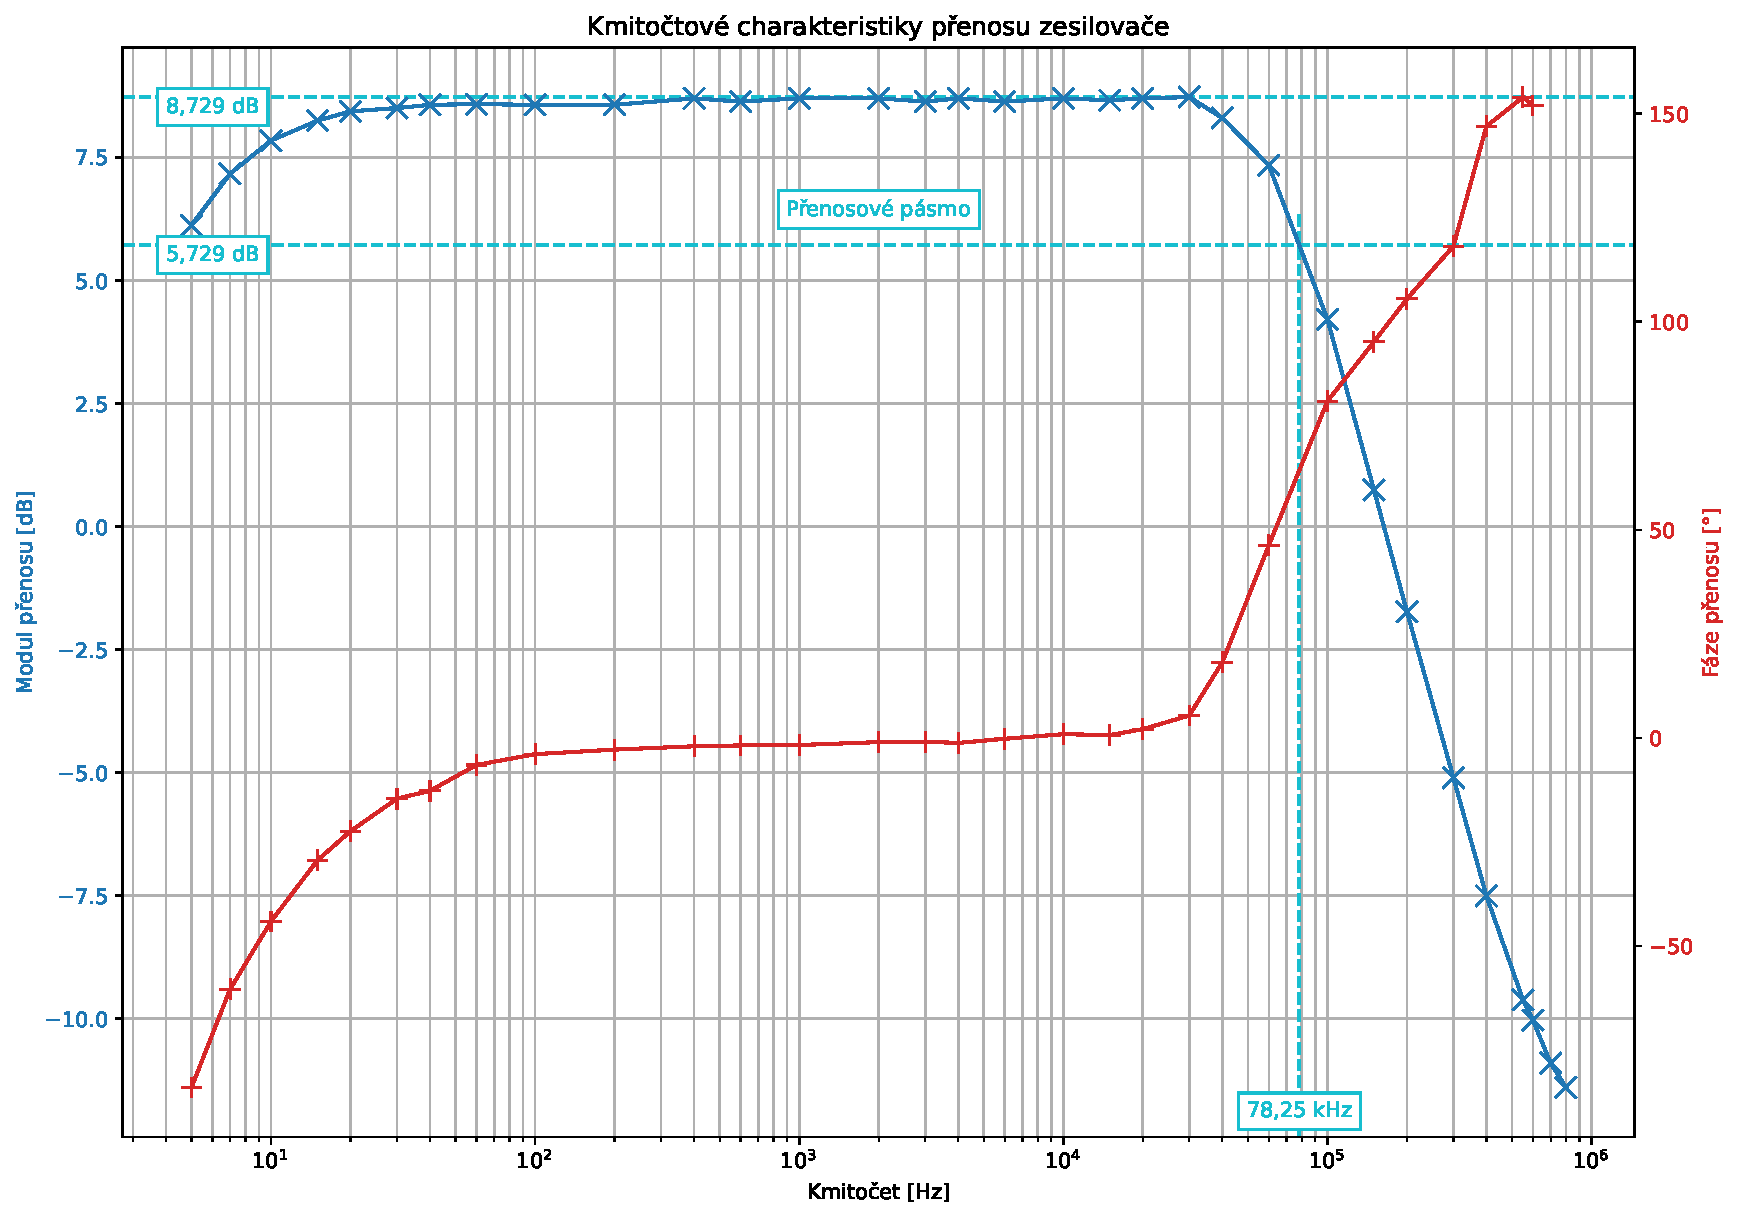
\includegraphics[width=\textwidth]{grafy/graf_kmitoctova_charakteristika.pdf}
    \caption{Kmitočtové charakteristiky modulu a fáze přenosu}
\end{figure}

\subsection{Příklady výpočtu}

\begin{enumerate}
    \item Rychlost přeběhu (Slew Rate)
    \begin{multline*}
        SR = \textcolor{teal}{\frac{\Delta u}{\Delta t}} = \frac{4,71 \, V}{3,17 \, \mu s} = \underline{\underline{1,485 \, V / \mu s}} \hfill
    \end{multline*}

    \item Amplitudy vyšších harmonických složek
    \begin{multline*}
        \textcolor{teal}{L_{dBV} = 20 \cdot log \left( U \right)} \hfill \\
        \ \ \ U_n = 10^{\cfrac{L_{dBV}}{20}} \hfill \\
        \ \ \ U_1 = 10^{\cfrac{L_1}{20}} = 10^{\cfrac{-12,5 \, dBV}{20}} = 237,1 \cdot 10^{-3} \, V = \underline{\underline{237,1\, mV}} \hfill
    \end{multline*}

    \item Celkové harmonické zkreslení
    \begin{multline*}
        THD = \textcolor{teal}{\frac{\sqrt{U_2^2 + U_3^2 + ... + U_n^2}}{\sqrt{U_1^2 + U_2^2 + U_3^2 + ... + U_n^2}} \cdot 100 \, \%} = \underline{\underline{0,289\, \%}} \hfill
    \end{multline*}

    \item Úroveň mezikanálových přeslechů
    \begin{multline*}
        L_p = \textcolor{teal}{20 \cdot log \left( \frac{U_{v \acute{y} st_2}}{U_{v \acute{y} st_1}} \right)} = 20 \cdot log \left( \frac{0,007 \cdot 10^{-3} \, V}{0,692 \, V} \right) = \underline{\underline{-99,90 \, dB}} \hfill
    \end{multline*}

    \item Dynamický rozsah (Signal to Noise Ratio)
    \begin{multline*}
        SNR = \textcolor{teal}{20 \cdot log \left( \frac{U_{v \acute{y} st_{max}}}{U_{v \acute{y} st_{min}}} \right)} = 20 \cdot log \left( \frac{0,292 \, V}{0,004 \cdot 10^{-3} \, V} \right) = \underline{\underline{97,26 \, dB}} \hfill
    \end{multline*}
\end{enumerate}

\section{Seznam použitých přístrojů}

\section{Závěr}

\end{document}